% needs IEEEtran.cls
%
\documentclass[10pt,journal,compsoc]{IEEEtran}
%\documentclass[conference,compsoc]{IEEEtran}

\usepackage{graphicx}% Include figure files
%\usepackage{bm}% bold math
%\usepackage{gensymb}
\usepackage{amsmath}
\renewcommand{\vec}[1]{\boldsymbol{#1}}
\usepackage{listings}
\usepackage{float}

\lstset{frame=tb,
  language=C,
  aboveskip=3mm,
  belowskip=3mm,
  showstringspaces=false,
  columns=flexible,
  basicstyle={\scriptsize\ttfamily},
  numbers=none,
  breaklines=true,
  breakatwhitespace=true,
  tabsize=3
}


%%%%%%%%%%%%%%%%%%%%%%%%%%%%%%%%%%%%%%%%%%%%%%%%%%%%%%%%%%%%%%%%%%%%%%%%%%%%%%%%
%%%%  Body of document follows...
%%%%%%%%%%%%%%%%%%%%%%%%%%%%%%%%%%%%%%%%%%%%%%%%%%%%%%%%%%%%%%%%%%%%%%%%%%%%%%%%
\begin{document}

\input{../source/qtdsp_title}
\IEEEtitleabstractindextext{%
\begin{abstract}
Consciousness can be considered a physical process occurring inside and outside of time simultaneously,
per spiritual traditions and modern QM theory (in its Bohmian interpretation),
using two-dimensional time.
In this model, quantum time emerges from non-local consciousness as it interacts with both worlds.
The relationship between the time dimensions provides a mechanism for apparent
noise arising from both our biological signaling and connection to a timeless divinity.
Algorithms are proposed for the demodulation of ubiquitous white and pink noise,
which could have hidden information content that instruments the
mind-body landscape and the interaction of eternal consciousness with the physical world.
This is key to solving the most pressing problem of our time, which is
``the totalitarian psychosis'' described by Carl G. Jung, or \emph{wetiko} as it's known
to indigenous peoples.
\end{abstract}


% Note that keywords are not normally used for peerreview papers.
\begin{IEEEkeywords}
Tao, noise, quantum time, relative time, consciousness, QTDSP.
\end{IEEEkeywords}}

\maketitle

%\tableofcontents

\section{\label{sec:level1}Two-Dimensional Time}

According to many spiritual traditions, including those that rely on
direct observation through meditation, the consciousness of humans, animals,
and all living things is a combination of the finite and the infinite,
existing both inside and outside of material reality.
Allowing more than one dimension of time theoretically supports this view
of existence beyond the material world.
The existence of non-local mind effects, since they hold up under serious
investigation \cite{Kelly}, provides a real impetus for multi-dimensional time.

Investigation of 2D time with an eye toward practical instrumentation has the
potential of bearing the kind of fruit necessary to
heal the schism between science and religion,
wipe evil off the face of the Earth,
and facilitate ascention of the planet.
Standing on the shoulders of giants provides a good starting point.

The Wheeler-DeWitt equation \cite{DeWitt} attempts to combine mathematically
the ideas of quantum mechanics and general relativity.
One of its implications is the ``problem of time'',
which is a conceptual conflict between general relativity and quantum mechanics.
Quantum mechanics regards the flow of time as universal and absolute, whereas
general relativity regards the flow of time as malleable and relative.

According to Wheeler-DeWitt, an observer outside of the universe
doesn't experience time. Page and Wootters \cite{Page} addressed this paradox
(time \textit{seems} real enough) by treating time as an emergent phenomenon
resulting from quantum entanglement.
Experiments \cite{Moreva} on entangled particles have bolstered the theory.

There are other takes on timeless universe models.
Aharonov's two state formalism of quantum mechanics has also been used
\cite{Lobo} to propose emergence of time from a timeless unus mundus
quantum-like space.
Jianfeng Li provides a good overview \cite{Jianfeng} of quantum mechanical
timeless consciousness.

There are two distinct types of time: emergent time, which emanates from the
structure of space-time and its metrics, and a causal time, indicating the flow
from the past to the future \cite{Brunet}. The time domains relate the
two models of Physics, QM and GR.
In the interest of having a nomenclature, we call one dimension of time
the quantum time domain and the other the relative time domain.
So, \textit{quantum time} and \textit{relative time}.
Relative time is the one with the arrow. 
This would be the same as ``absolute time'' in some parlance, but since we don't
know that ``the clock'' has been running at a constant rate since the Big Bang
``relative time'' seems a better fit and pays homage to relativity.

The hard problem of consciousness \cite{Chalmers} is that of explaining the
relationship between physical phenomena, such as brain processes,
and experience.
Experiments in non-locality \cite{Achterberg} find that the mind extends beyond
the skull. Where is the mind, inside space-time or outside?
The evidence suggests it is both.

Our everyday experience is that ``clock time'' is the reference frame,
although it could just as well be that quantum time is the existential norm
and the ``clock time'' universe is a special case.
We take the view of quantum time observed from within the universe, with
the observation being an act of quantum entanglement caused by consciousness.

\subsection{Quantum Time and Consciousness}

In the field of ``quantum biology'',
there are many examples of biological systems exploiting quantum effects.
One could suppose that nature would evolve to use quantum time.

The physical vacuum, a substrate for quantum interactions,
is a natural mechanism for biological systems to have evolved to utilize.
This pantheistic view allows for consciousness as the ground state of being.
Consciousness is the interaction between the physical vacuum and biology which
facilitates communication at any physical scale, from DNA to organism.

This provides an important signaling mechanism for consciousness in beings such
as paramecia or slime molds, which exhibit conscious behavior but are too small
for consciousness to arise from the network effects of neurons or ganglia.

One way to relate the two time dimensions is with a scale-invariant geometry
that exploits the simplicity of self-similarity.
As Mandelbrot \cite{Mandelbrot} pointed out, relatively simple fractal
mathematics underlie many complex natural phenomena.
As it turns out, this exponential relationship between $\tau$ and $t$
is a key enabler of signal transformations.

For it to be scale invariant,
we use an exponential growth model for quantum time.

\begin{equation} \label{eq:pink}
\tau \propto e^{\epsilon t}
\end{equation}

The mechanics of signal generation can be considered in the context of
quantum time.
This arrangement lends itself to information flow, utilized by nature,
between the time and timeless domains.

Resonance is treated as a physical phenomenon occurring in quantum time $\tau$.
A resonant frequency in $\tau$ is equivalent to an exponential chirp in $t$.
This dynamic emergence of time should produce small but detectable artifacts.
The stream of consciousness is treated as emerging from a probabilistic field
on an exponential time scale rather than time abruptly appearing from nothing.

Biological systems evolve to minimize the expenditure of energy. Resonances
(field analogs of electrical and mechanical ringing) require a small energy
input to keep them going, assuming a reasonably high Q. It stands to reason
that biological systems would use field resonances in the physical vacuum
(the exact nature of the field needs not be understood)
to transmit consciousness information efficiently.

In other words, there is a hypothetical basis for the notion that
``It's all vibrations''.
The vibrations occur in quantum time,
so their signal artifacts produce a noise spectrum.
Of course, nature is never simple. There could be other dimensions at play or
even backward time effects providing the excitation for the resonance.
Since we're only looking for artifacts, the details aren't as important
as verifying the existence of the artifacts in the first place.

The signals that encode this information can be demodulated from ``noise''.
We live in a world of electronic noise, which usually caused by various physical mechanisms.
By digitizing and processing this noise in a warped time domain,
consciousness information may be extracted using traditional detection technologies.

\section{Exponential Flicker Noise}

Flicker noise (or 1/f noise), has a power spectrum proportional to
$1/f^{\alpha}$, where $\alpha$ is between 0.7 and 1.4.
It's a type of noise prevalent in many natural systems.
Flicker noise \cite{Milotti} is seen in music, seismic data, EEG and ECG data,
and electronic devices.
Some of the more popular explanations for the 1/f spectrum are:
\begin{itemize}
	\item A superposition of relaxation processes.
	\item Carrier mobility fluctuations through Coulomb scattering.
\end{itemize}
There are a good number of hypotheses for 1/f noise, to which we add one more:
\begin{itemize}
	\item The superposition of exponential chirps.
\end{itemize}
An exponential swept-sine signal with constant amplitude has a power spectrum
\cite{Novak} that is constant-slope (on a log-log plot) at roughly -6dB
per octave, curiously similar to a flicker noise power spectrum.
This is independent of ``warp factor'' $\omega$.
\begin{equation}
Signal \propto sin(k \cdot e^{\omega t})
\end{equation}

\subsection{Exponential White Noise}

White noise has a flat power spectrum.
In a white noise model of quantum time, chirps start at 0 and asymptotically
approach a final frequency as quantum time merges into relative time.

\begin{equation} \label{eq:white}
\frac{1}{\tau} \propto (1-e^{-\epsilon t})
\end{equation}

In other words, the consciousness signal emerges from a domain of infinite time.
The power drops off at the same rate frequency increases,
resulting in a flat spectrum from DC to $f_0$.

\begin{equation}
f = f_0 \cdot (1-e^{-\epsilon t})
\end{equation}
\begin{equation}
p = p_0 \cdot e^{-\epsilon t}
\end{equation}

$f_0$ would be millimeter wave (such as 60 GHz oxygen resonances) and higher.
Terahertz (mostly in the 600 THz range) oscillations in tubulin \cite{Craddock}
correlate with anesthetic potency, which opens the possibility that
tubulin oscillations are carriers of consciousness information.

The chirp would mix with carrier $f_0$ to produce a downward chirp
(assuming the signal is moving forward in time)
with power dropping with frequency,
which flattens out the spectrum so it's still white.
The resulting chirp signal is more practical due to the shortness of the
time the chirp itself spends in a bandwidth that lends itself to detection.

The amplitude droop may be compensated for in the input warping stage.
White noise follows the same rules as pink noise except for the spectral bias.

\subsection{Information in the Noise}

Since exponential chirps are bounded in time, a single chirp has a finite
existence. It corresponds to a discrete impulse in the relative time domain,
or one symbol of information.
The idea of consciousness as time quanta may be useful here.
The act of being is a stream of consciousness that has corresponding streams
of pulse-coded information, a kind of informational counterpart to DNA.
The impulse stream may be decoded for its information content.
The detection of an impulse stream itself is valuable,
regardless of our initial ability to decode it, because useful information
can be mined from its distribution of $\omega$ values.

Consciousness quanta have a foundation in Penrose and Hameroff's
``Orch OR Theory'' \cite{Hameroff}.
In objective reduction, the divergence of quantum superposition in the
underlying structure of the universe builds to the point of collapse,
or objective reduction of the quantum state.
Each collapse is a moment of conscious experience.
In ``Orch OR'', EEG data is a macro view of these moments.
EEG has both a flicker noise spectrum and frequency peaks that correspond
to ``Orch OR'' collapse.
There is already much scientific data (such as EEG and ECG studies) in the
public domain, ready to analyze.
The experimental costs are low: mostly computer hardware.

Overlapping chirps can be re-sampled and self-correlated to construct a relative
time domain signal for one or a multiplicity of $\omega$ values.
A sweep of $\omega$ can be used to construct a ``warp spectrum'' (for example,
on a computer display), useful for finding quantum-time signals.
This would be analogous to waterfall-style spectral analysis, with frequency
replaced by warp factor.

To establish a notation and unit of measurement for quantum frequency,
let the ``warp factor'' $\omega$ be in units of $e$, the
mathematical constant derived by Leonhard Euler in the 1720s, per unit time.
The pronunciation may be ``e's per second'' for e/s, for example.
We propose ``len'' for the unit name of e/s, after Leonhard.
Some scale factors to other units: 0.69 lens is one octave per second,
2.3 lens is one order per second, and 0.48 lens is one golden mean
$(\Phi=1.618:1)$ per second.
Note that a len is very close to twice the Golden Ratio,
so one must be careful when making assumptions about Golden Ratio relationships
in nature.

%%%%%%%%%%%%%%%%%%%%%%%%%%%%%%%%%%%%%%%%%%%%%%%%%%%%%%%%%%%%%%%%%%%%%%%%%%%%%%%%
\subsection{Spiral Conceptual Model}

\begin{figure}[h]
	\centering
	\includegraphics[width=0.7\linewidth]{../source/spiral_e}
	\caption[Quantum to Relative Time Relation]{Log polar plot of exponential chirp}
	\label{fig:spiral}
\end{figure}

Resonant signals in the quantum time domain can be re-mapped to relative time
and demodulated by correlating a series of fast exponential chirp
transforms, allowing analysis and data mining using modern data
processing technologies such as AI-based pattern recognition.

The correlation effect can be visualized as a spinning logarithmic spiral
illuminated by a strobe light. When the strobe frequency matches the rate
constant of the spiral(s), it appears to be standing still.
Otherwise, it's a blur.

The relationship between quantum time and relative time can be thought of as a
2D plot in log-polar format.
Log-polar format renders a logarithmic spiral as a linear (Archimedean) spiral.
The spiral's radius is $\rho = k\theta$, where $k$ is a rate constant.
$\rho$ can represent either time or frequency by flipping the sign of $k$.
For purposes of signal processing, let $\rho$ represent log frequency and
$\theta$ relative time.

Log-polar mapping has proven useful in machine vision \cite{Bonmassar}
because it approximates the primate visual map \cite{Schwartz}.
Humans are visual thinkers, so their waking consciousness should map onto the
log-polar structure of quantum time signaling.

Fig.~\ref{fig:spiral} plots an exponential chirp in log-polar format.
A line can be drawn outward from the center of the spiral, crossing it at
multiple points.
The line rotates clockwise (in the case of downward chirp) at a step size
(from $t_1$ to $t_2$) corresponding to the oversampling rate.
For example, if the oversampling rate is 36 (each input value is used 36 times),
the step size is $10^{\circ}$.
Each angular sweep of the unit circle
(beginning and ending at line $t_1$ or $t_2$)
represents the input to a version of the Mellin transform called the
``Exponential Chirp Transform'' (ECT) \cite{Bonmassar}, which is
basically a FFT with time-warped input.

The transform's frequency domain output is along line $t_1$ or $t_2$ from
approximately $\rho$ = 0 to Fs/2, where Fs/2 (the Nyquist frequency)
is shown by the dashed circle.
The radius of the circle represents the approximate bandwidth of the system.
Not all of the circle is used: Anti-aliasing cuts off before Fs/2, while signal
near the center is too spread out to be useful.

The ECT time-warps the chirp signal, which represents a single ``quantum tone".
In the $360^{\circ}$ sweep at line $t_1$,
the chirp is time-warped to a tone F1 in relative time.
A time $t_2-t_1$ later, at line $t_2$,
it's time-warped to a tone of frequency F2.
All time warping is exponential.
Note that ``exponential time warping'' is different from dynamic time warping,
a popular means of pattern-matching mostly linear signals.

A convenient side effect of time warping is to transform interference
(periodic signals) into wideband noise.
The usual frequency peaks of EEG and HRV are thus discarded.

Quantum time, being logarithmic, has the property of frequency going as
$-\tau$ rather than $1/t$.
To change between time and frequency, just flip the sign of the exponent.
Tones are mirror images of time.
Signal processing is more convenient in terms of frequency,
so that is the focus of this paper.

%%%%%%%%%%%%%%%%%%%%%%%%%%%%%%%%%%%%%%%%%%%%%%%%%%%%%%%%%%%%%%%%%%%%%%%%%%%%%%%%
\subsection{\label{sec:level1}Quantum Time DSP}

The basic data flow of signal conversion from one time domain to another
$(\tau \leftrightarrow t)$ is shown in Fig.~\ref{fig:sled}.
The conversion algorithm slides along the input and output data streams,
forward in time.
Data is processed in overlapping chunks.
In other words, after a block of processing,
the sliding part of Fig.~\ref{fig:sled} shifts slightly to the right.
In proportion to the amount of shift,
new input stream is exposed and new output stream is completed.
The I/O streams are low-bandwidth compared to the compute-intensive
processing block.

\begin{figure}
	\centering
	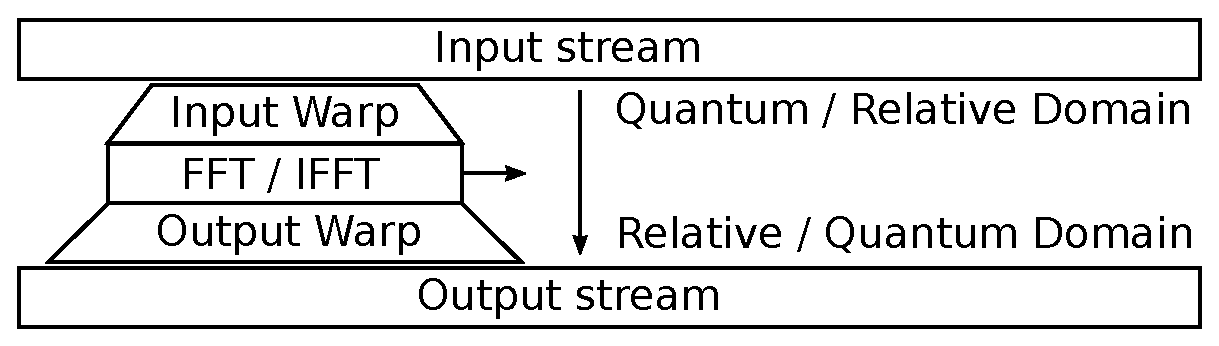
\includegraphics[width=0.95\linewidth]{../source/sled_e}
	\caption[Quantum to Relative Time Translation Flow]{Inter-domain data flow}
	\label{fig:sled}
\end{figure}

There are two use cases: demodulation and modulation.
For demodulation $(\tau \rightarrow t)$, the input stream is in the quantum
time domain and the output stream is in the relative time domain.
The downsampler decimates the input by 1:m, where decimation factor m is
exponentially swept upward from or downward to 1.0.
The ``warp factor'' is the growth rate in m.
The input stream consists of real numbers.
The FFT performs a real-to-complex FFT to produce a warped spectrum which is
treated as a time-domain envelope of magnitude and phase information.
To un-warp the spectrum, the upsampler interpolates it by 1:m where decimation
factor m is exponentially swept upward to or downward from 1.0.
The output stream consists of vectors that are many accumulations of overlapped
upsampler results.

For modulation $(t \rightarrow \tau)$, the input stream is in the relative time
domain and the output stream is in the quantum time domain. The downsampler
decimates the input by 1:m, where decimation factor m is exponentially swept
upward from or downward to 1.0 and the resulting spectrum ranges from about
N/5 to N/2.
The ``warp factor'' is the growth rate in m.
The input stream consists of complex numbers.
The IFFT performs a complex-to-real IFFT to produce a time domain
envelope. To warp the it, the upsampler interpolates it by 1:m
where decimation factor m is exponentially swept upward to or downward from 1.0.
The output stream consists of many accumulations of overlapped upsampler results.

The usual use case is demodulation.
Modulation could be for testing, reconstruction or extrapolation of a signal,
or modulation of an energy source for yet unknown applications.


\section{QT Demodulation}

\begin{figure}
    \centering
    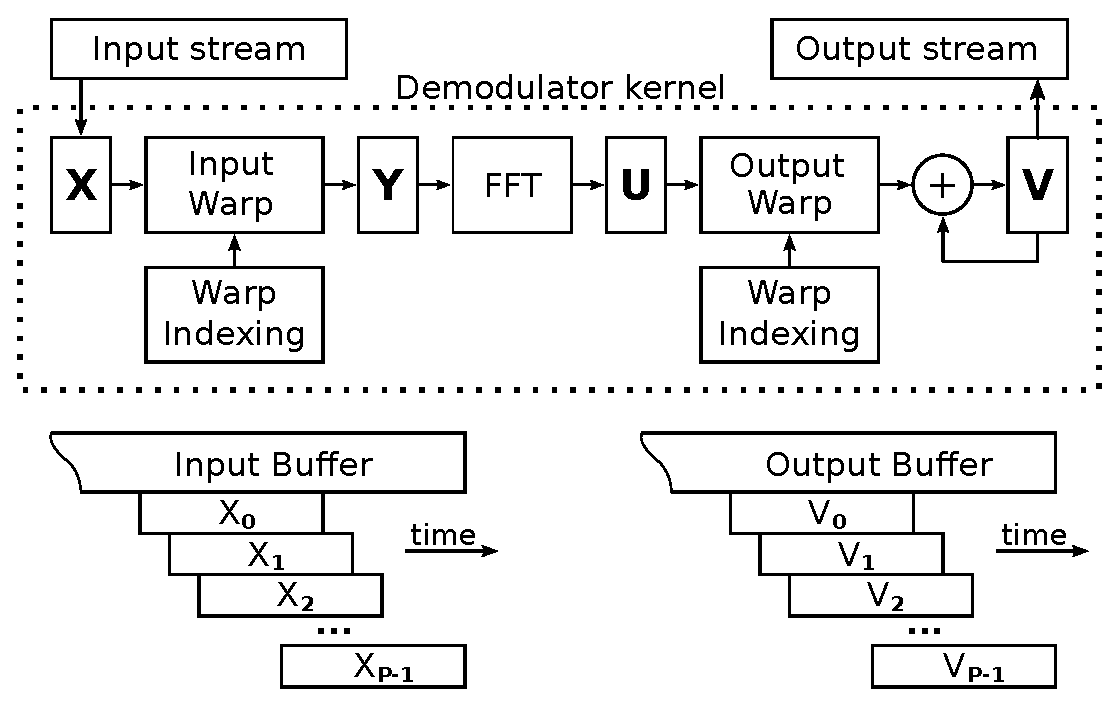
\includegraphics[width=0.95\linewidth]{../source/demod_e}
    \caption[Quantum to Relative Time Demodulation]{Demodulation data flow}
    \label{fig:demod}
\end{figure}

Due to the low I/O bandwidth, the algorithm lends itself to parallelism without
the complexity of high-speed signaling or memory management.
A low-cost ASIC would be feasible for consumer applications.

The mathematics of signal conversion, besides FFT, is mainly College Algebra.
The algorithm can be coded by a typical programmer or engineer with some help
from the following derivations.

%%%%%%%%%%%%%%%%%%%%%%%%%%%%%%%%%%%%%%%%%%%%%%%%%%%%%%%%%%%%%%%%%%%%%%%%%%%%%%%%
\subsection{Input Warping}

The downsampling process of Fig.~\ref{fig:demod} translates the sample pitch of
X to the sample pitch of Y using an exponential sweep.
In the industry, this is known as exponential time-warping.

An exponential chirp sweeps from $f_0$ to $f_1$ in a time T.
M points of X get mapped onto N points of Y, where $M < N$.
Regardless of the sign of $R$, the input warp shifts the corresponding chirp
to the lesser of $f_0$ and $f_1$. The highest frequency component in the input
is $frac{F_S}{2} \cdot frac{1}{1 + |R|}$. Input interpolation produces noise
artifacts, as you would expect. 
As it turns out, they get spread broadly across the spectrum above the region of
interest. Those FFT outputs are ignored.
That's fabulous news, because it removes any motivation for much more
compute-intensive resampling algorithms. Warping may be kept simple and fast.

Let R be a scaled version of $\omega$ for use in the exponential warp and
$\alpha$ the X input sample rate in samples per second.
Given a particular R and N, M and $\omega$ may be calculated.
Let $\epsilon = (f_1/f_0)^{1/T}$. The frequency with respect to time is:
\begin{equation}  \label{eq:fvsf0}
f = f_0 \cdot e^{\epsilon t}
\end{equation}

\subsubsection{Math}

The period of the incoming chirp changes exponentially with index n of $X[n]$.
Let $y = e^{|R|/N}$ be the pitch that accumulates along X.
It has units of ``e's per sample''.
As a scale factor, let $\omega = \frac{\alpha R}{N}$,
in units of ``e's per second'' e/s.
M is the number of input samples warping onto N points.
To time-warp the input, let N be a sum of M segments whose size starts at 1 and
get compressed exponentially. 
The calculation of M starts with a geometric progression in Eq. \ref{eq:M_N0}.

\begin{equation}  \label{eq:M_N0}
N = \sum_{k=1}^{M} e^{-|R| \cdot (k-1)/N} = \frac{1 - e^{-|R| \cdot M/N}}{1 - e^{-|R|/N}}
\end{equation}

\begin{equation}  \label{eq:M_N}
M = \frac{-N}{|R|} \cdot\ ln\left( 1 - N(1-e^{-|R|/N}) \right)
\end{equation}

Re-sampling is done on N points (of Y) at a time where the respective indices of
X and Y are $\delta$ and i.
X is swept from X[0] to X[M-1] or X[M-1] to X[0].

Interpolating from a fractional X index can be done by cubic interpolation
using a Catmull-Rom spline. 
Linear interpolation may be used although it's a little noisier.
The noise extra noise might not make a difference.
Cubic interpolation is a very useful and interesting technique in computing,
so let's touch on that anyway.

Given four points $y_0, y_1, y_2, y_3$, a cubic polynomial describes the curve
passing through all four points, whose slope matches up between adjacent segments.
With $x$ ranging from 0 to 1 indexing the point on $[y_1, y_2]$.

\begin{equation}  \label{eq:cubic}
f = a_0 \cdot x^3 + a_1 \cdot x^2 + a_2 \cdot x + a_3
\end{equation}

\begin{gather*} 
a_0 = -0.5y_0 + 1.5y_1 - 1.5y_2 + 0.5y_3;\\
a_1 = y_0 - 2.5y_1 + 2y_2 - 0.5y_3;\\
a_2 = -0.5y_0 + 0.5y_2;\\
a_3 = y_1;
\end{gather*}

The time span is from 0 to i/N where i sweeps from 0 to N-1 and N is the number
of samples.
Let $\lambda$ be the sample pitch of X.
It will increase or decrease exponentially and should have a maximum value of 1.

This causes a chirp of matching R to be re-sampled to the upper frequency
(either $f_0$ or $f_1$ depending on the sign of R).
Given output index i, input sample index $\delta(i)$ is the accumulated sum of
$\lambda(i)$ when $\lambda$ starts at 1.0 and increases exponentially
or starts at $e^{M \cdot R/N}$ and decreases exponentially.
The exponential sweep can be implemented with a multiplier.
For each step:
\begin{equation}  \label{eq:lambda}
\lambda = \lambda + (\lambda\cdot\Lambda)
\end{equation}

The initial value of $\lambda$ is $e^{M \cdot R/N}$ when $R>0$; otherwise, it's 1.
The ``repeated multiply'' approach to exponential sweep is nearly base $e$,
but it needs a small correction factor to hit $e$.
Setting $e^R = (1 + \Lambda)^N$,
\begin{equation}  \label{eq:lambdaApprox}
\Lambda = e^{R/N} - 1
\end{equation}

A sample C implemention of the warp transform using cubic interpolation is:

\begin{verbatim}
void Warp(
  float* out,        // output stream
  float* in,         // input stream
  int length,        // points in output stream
  double delta,      // starting input index, 0 to 1
  double pitch,      // exponential input sample pitch
  double lambda,     // rate of change of pitch
  double amplitude,  // starting amplitude
  double fcomp)      // decay rate of amplitude
{
  float y0 = *in++;
  float y1 = *in++;
  float y2 = *in++;
  float y3 = *in++;
  // coefficients for first y1-y2 segment of the curve
  float a0 = -0.5 * y0 + 1.5 * y1 - 1.5 * y2 + 0.5 * y3;
  float a1 = y0 - 2.5 * y1 + 2.0 * y2 - 0.5 * y3;
  float a2 = -0.5 * y0 + 0.5 * y2;
  float a3 = y1;
  for (int i = 0; i < length; i++) {
    float x = delta; // between 0 and 1 on y1-y2 path
    float sum = x * (x * (x * a0 + a1) + a2) + a3;
    *out++ = sum * amplitude; // deemphasize low end
    delta += pitch;
    if (delta >= 1.0) {
      delta -= 1.0;
      pitch += pitch * lambda;
      amplitude += amplitude * fcomp;
      y0 = y1;       // stepped into the next segment
      y1 = y2;
      y2 = y3;
      y3 = *in++;
      a0 = -0.5 * y0 + 1.5 * y1 - 1.5 * y2 + 0.5 * y3;
      a1 = y0 - 2.5 * y1 + 2.0 * y2 - 0.5 * y3;
      a2 = -0.5 * y0 + 0.5 * y2;
      a3 = y1;
    }
  }
}
\end{verbatim}

\begin{figure}
    \centering
    \includegraphics[width=0.95\linewidth]{../source/xbuf_e}
    \caption[X buffer usage]{X buffer usage}
    \label{fig:xbuf}
\end{figure}

Oversampling would normally use a sliding window on a circular buffer sized as
a power of two to allow pointer wrapping by bitwise-and.
Fig.~\ref{fig:xbuf} shows the memory layout of $X$.
After a block of processing, $\alpha\Delta$ input samples are concatenated to
$X$ and the index of $X_0$ is offset by $\alpha\Delta$,
where $\Delta$ is the time interval of the blocks.

%%%%%%%%%%%%%%%%%%%%%%%%%%%%%%%%%%%%%%%%%%%%%%%%%%%%%%%%%%%%%%%%%%%%%%%%%%%%%%%
\subsection{FFT}

After X is time-warped into Y, Y is processed by a Fast Fourier Transform and
converted to data set U containing N/2 frequency bins. Y and U may share the
same physical memory if the FFT is performed in place.
The output of the FFT is converted to the square of the magnitude,
so square root is not needed.

A window function $w(n)$ is applied to Y before performing the FFT.
Hann and Nuttall functions are both good functions, with a tradeoff between
peak spreading and dynamic range. The Hann function is:

\begin{equation}
w(n) = \frac{1}{2}\left(1 - cos\left( \frac{2\pi n}{N-1} \right)\right)
\end{equation}

A DIT FFT is the usual choice for RFFT since bit reversal is easier at the input.
With an RFFT, you get twice the outputs given real-only input.
Adjacent input samples are grouped as pairs, with even samples as real and odd
samples as imaginary components of the complex input points.
After a CFFT is performed, a separation step doubles the output size.

%%%%%%%%%%%%%%%%%%%%%%%%%%%%%%%%%%%%%%%%%%%%%%%%%%%%%%%%%%%%%%%%%%%%%%%%%%%%%%%%
\subsection{Output Warping}

U is upsampled to form time-domain signal V.
Let $\epsilon$ and j be the respective indices of U and V.
For every index $\epsilon$ of U, the corresponding frequency can be normalized
to a fraction $(\gamma)$ of $Fs/2$.

Hardware-wise, it's much easier to work in terms of exponents than logarithms,
so the preferred re-mapping (another exponential time-warping operation)
extracts $U[\epsilon]$ from a linear progression of $V[j]$.
Warp indexing uses the relation:
\begin{equation}
\epsilon = \left(\frac{N}{2}-1\right) e^{\omega(t - \tau)}
\end{equation}

Time $t$ (scaled to match the output stream's sample rate) sweeps from $\tau$
in the opposite direction of R's sign,
causing the exponent to start at 1 and decay downward.

$j$ sweeps downward from $\gamma(N/2-1)$.
Index $\epsilon(j)$ is independent of R.

\begin{equation}  \label{eq:eps_j}
\epsilon(j) = \gamma \left(\frac{N}{2}-1\right) e^{-kj/N}
\end{equation}

The desired difference between $\epsilon(0)$ and $\epsilon(1)$ in
Eq. \ref{eq:eps_j} is $1$. $\epsilon(0) = \gamma(N/2 - 1)$.

\begin{equation}
\epsilon(1) = \gamma(N/2 - 1) - 1 = \gamma(N/2 - 1) e^{-k/N}
\end{equation}

This gives a $k$ of approximately $2/\gamma$. The exact value is:

\begin{equation}
k = N \cdot ln \left( \frac{N-2}{N-2-(2/\gamma)} \right)
\end{equation}

As a sanity check of Eq. \ref{eq:eps_j}, $\epsilon(j)$ starts at
$frac{F_S}{2} \cdot frac{1}{1 + |R|}$.
It decays toward 0 but will never get there.
The number of elements in W memory is slightly less than N/2 to allow some I/O
headroom. Due to the limited size of W memory,
the lowest frequency is about $(1/e)$ of the highest frequency,
leaving the lower $\approx37$\% of the spectrum unused when $\gamma=1$.

The exponential decay of $\epsilon$ can be handled by repeated multiplication,
one per $U[\epsilon]$ fetch.
The exponential sweep needs a small correction factor to have a base of exactly
$e$.
%\frac{N}{2} \cdot (1 - e^{-k})
Setting $e^{-k} = (1 + \zeta)^{N}$,
\begin{equation}
\zeta = e^{k/N} - 1
\end{equation}

Let $H_X$ be the integer number of new X samples per conversion.

Let $H_V$ be the real number of output samples per conversion.

\begin{equation}  \label{eq:hv}
H_V = H_X \cdot \frac{|R|}{k}
\end{equation}

Since $\epsilon$ is always positive, the upchirp case of $R>0$ needs to have its
j index mirrored by using V[v-j], where v is the maximum j such as (15/32)N.
The upsampler output is added to V memory as described below, indexed from the
top or bottom of the active region of V.

%%%%%%%%%%%%%%%%%%%%%%%%%%%%%%%%%%%%%%%%%%%%%%%%%%%%%%%%%%%%%%%%%%%%%%%%%%%%%%%%
\subsection{Correlation}

Warped U is added to output buffer V by RMS summation,
staggered in time (by $H_V$ samples) for each processing block.
When the downsampler's R value matches the chirp rate of an incoming chirp,
multiple peaks in the warped FFT output correlate in the output stream to
produce a corresponding output pulse in the V stream.
A more complex signal such as overlapping and/or modulated chirps will produce
pulse trains and/or modulation envelopes in the V stream.

\begin{figure}
    \centering
    \includegraphics[width=0.99\linewidth]{../source/wbuf_e}
    \caption[W correlation]{Correlation of V}
    \label{fig:wbuf}
\end{figure}

Fig.~\ref{fig:wbuf} shows the output correlator, another view of buffer V.
The output stream flows from left to right,
being initialized to 0 outside the accumulation region.
After $U_\epsilon$ is added to V, the $V_0$ index moves $H_V$ points
to the left, leaving $H_V$ newly minted output points.

Elements of V are accumulated squares of magnitudes.
An attempt was made to accumulate vectors,
with the idea that the phase rotations might sync up,
but it didn't work in simulation.
So, angle data from the FFT is discarded.

\input{../source/qtdsp_demodp}
%\input{../source/qtdsp_mod}
\section{Testing the Demodulator}

The demodulation algorithm was tested by coding the algorithm in C.
The test app uses OpenGL and GLFW3 to provide a user interface and NVIDIA's
CUDA SDK to provide DSP power for the transform.

The software has a dependency on NVIDIA GPU cards.
The magic of GPUs lies in an architecture that efficently streams DRAM bursts
into and out of many CPU cores that operate in parallel.
The application operates on many values of R concurrently.
The development PC had a GTX 1080 graphics card.
Newer graphics cards such as the GTX 1660 ti offer nearly the same performance
at much lower cost: The DRAM bus isn't as wide but it uses a faster clock.
Look for a wide (such as 192-bit) memory bus and GDDR6.

With the GTX 1080, the CUDA-based algorithm was about 15 times as fast as an
FFTW-based version running on a single thread of a 3 GHz CPU core.
Running the algorithm in many threads on an expensive CPU could bring the
performance more in line with GPU performance,
but more likely is that memory bandwidth limitations will keep a CPU-based
solution slower than the GPU-based version.
Some of the higher end GPUs use stacked-die memory to provide much higher
bandwidth, so GPUs provide a real performance upgrade path.

The spectrogram consists of a range of R values spread vertically with time on
the horizontal axis.
Since the number of output points vary with R, time is normalized to the left 
edge of the image. At the left edge, the same amount of total time has elapsed
for each row of pixels.

\subsection{Spectrogram of a test chirp}

Figure \ref{fig:chirpTest1} shows a spectrogram image of a noisy
negative-chirp (R = -0.5) test signal with R on the vertical axis.
$R=-0.4$ is at the top and $R=-0.6$ is at the bottom.
A test signal was used to demonstrate detection of a chirp at
$R=-0.5$ and $N=4096$.
The chirp amplitude is 1/10 of the noise amplitude.
\begin{figure}
  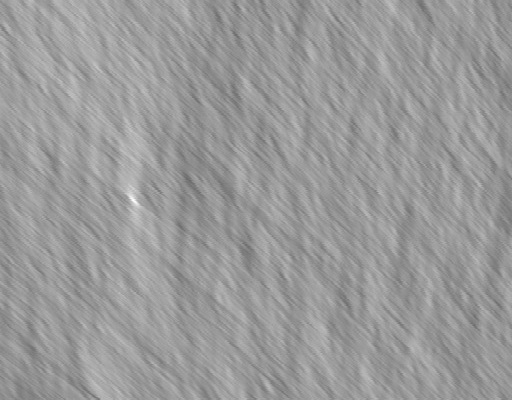
\includegraphics[width=\linewidth]{../source/chirp42m.jpg}
  \caption{Chirp power $(R<0)$ 20dB below noise.}
  \label{fig:chirpTest1}
\end{figure}

The noise produces a kind of slate or sandstone texture.
The white spot is the test chirp.
An oversample factor of 64 seems to be optimal.
Oversampling is the number of times an X input point is used in overlapping
operations. For example, 64 new input points for N = 4096.
Lower oversample factors leave more visible (patterned) artifacts.
Higher ones produce about the same smoothness with more computation load.
They don't really increase sensitivity.
Higher N mostly increases resolution and to some extent sensitivity.

White, pink, and brown noise (without the test chirp) has about the same 
appearance noted above.

\subsection{Spectrogram of music}

The first 2.5 minutes of Bach's Toccata and Fugue in D minor seemed like a good
test of tone-rich music. Organ notes are rich in harmonics.
The other test was the Surfaris ``Wipe Out'', another instrumental piece with
rich harmonics. Both were resampled to 22050 SPS.

\begin{figure}
  
\includegraphics[width=\linewidth]{../source/bach220.jpg}
  \caption{Bach's Toccata and Fugue in D minor.}
  \label{fig:bach220}
\end{figure}

Figure \ref{fig:surfariswipeout} illustrates the texture of a periodic waveform.
Tones appear as wideband noise in the FFT output. 
They can produce wide but faint lines in the output.

\begin{figure}
  
\includegraphics[width=\linewidth]{../source/surfariswipeout.jpg}
  \caption{The Surfaris Wipe Out.}
  \label{fig:surfariswipeout}
\end{figure}


\subsection{Spectrogram of an EEG signal}

EEG data was downloaded from the Sleep Spindles Database, excerpt 2.
Its web link is broken, but the data is in the wild.
Figure \ref{fig:excerpt2} shows the spectrogram during stage 2 sleep.

The spectrogram looks different from synthetic noise. 
It has the slate-like texture of synthetic noise but with ``scratches'' and ``hair''
that give a different appearance.

\begin{figure}
  
\includegraphics[width=\linewidth]{../source/excerpt2.jpg}
  \caption{EEG of a test subject in stage 2 sleep.}
  \label{fig:excerpt2}
\end{figure}

\begin{figure}
  
\includegraphics[width=\linewidth]{../source/wokessd.jpg}
  \caption{EEG of a test subject waking up from sleep for about 30 seconds.}
  \label{fig:wokessd}
\end{figure}

Although visual interpretation at this point is like reading tea leaves,
a trend that seems to be at play is that the warp factor, $\omega$, is not
constant. It changes exponentially, forming sloped (but mostly straight) lines
in the output.
These lines overlap in time and have different slopes.
Sometimes the slope shifts from positive to negative, through vertical.
Sometimes it seems a line with a slope will have a line near it with the
sign of its slope flipped.

The exponential emergent time model is much more complex than initially thought.
You would think we were dealing with nature.
The signals we're looking at aren't self-similar fractals.
The most computationally feasible means of decoding is probably to stick with
the exponential chirp transform model and post-process the 2D spectral image.
The transform depends on self-similarity in the time warping, which seems to
limit it to a power function. 

Rather than ``fix`` the transform, it should be easier to 
look for lines in the spectrogram.
It may be useful to keep in mind that an FM-modulated signal will produce
multiple parallel lines. The intensity of the lines would be reminiscent
of the frequency spectrum of a typical FM signal.

\section{Summary}

Signals that appear to be pure noise may contain hidden signals regarding non-local consciousness.
These signals could be analyzed to ``instrument the soul''.
Follow-up work to be done includes:

\begin{itemize}
	\item Add features to the QTSA app to facilitate signal identification.
	\item Analyze existing experimental data to search for new signals.
	\item Develop new sensor technologies using quantum and spin effects.
\end{itemize}

The social impetus for such work is to repair the dysfunction introduced by
new technologies such as social media and pseudo-anonymous communications.
Instrumenting the soul would provide a new way of interacting that is completely open and honest.
Solving the trust problem would be a boon to economies across the globe.


\bibliographystyle{IEEEtran}
\bibliography{IEEEabrv,../source/qtdsp}

\end{document}

